\chapter{Evaluation of the Cloud Scheme}

\section{Introduction}

In this chapter, the simulated climatology from the simple cloud scheme described in \chapref{chp:simple_cld_scheme} is presented here. \secref{sec:exp_setup_and_dataset} introduces the experiment setup and data sets used in this chapter. The evaluation will focus on features of cloud fraction, cloud water path and cloud radiative effects, including their vertical profile (if any), spatial pattern, zonal mean structure and seasonal cycles.


\section{Experiment setup and data sets}
\label{sec:exp_setup_and_dataset}

\subsection{Experiment setup}

Our simulations are AMIP-type, that is they follow those used in the Atmospheric Model Intercomparison Project. They are performed with a realistic Earth-continental configuration following \citet{Thomson2018} (which is derived from the ERA-Interim land mask and topography \citep{Dee2011}) and at a horizontal resolution of T42 (roughly 2.8$^\circ$ $\times$ 2.8$^\circ$) with 25 vertical levels. The sea surface temperature is fixed at AMIP climatology \citep{Taylor2000sea}, which is annually repeating but seasonally varying. The sea ice data is also from AMIP, but is averaged over all years and months to obtain an annual mean distribution, as in \citet{Thomson2018}. The albedo in sea ice regions increases linearly with the sea ice concentration with the maximum of 0.7. The surface albedo of the other parts except the sea ice is fixed as 0.11. The insolation includes a seasonal and diurnal cycle, with a solar constant of 1360 Wm$^{-2}$. The convection parameterization used in this study is the simplified Betts--Miller scheme from \citet{Frierson2007}. 

The SOCRATES (Suite of Community Radiation Codes based on Edwards \& Slingo) radiation scheme \citep{Edwards1996, Manners2015} is employed for the radiation transfer calculation as in \citet{Thomson2019}. Spectral files with 9 longwave bands and 6 shortwave bands are used, which are those used in the Unified Model's Global Atmosphere version 7 \citep{Walters2019}. The cloud fraction, effective radius of cloud particle and liquid water mixing ratio in each grid are passed to it, then the radiation fluxes under all-sky and clear-sky conditions are obtained, which are used to analyze the energy balance and to calculate the cloud radiative effect \citep{Ramanathan1989, Li2017} at the TOA.

In order to compare the roles of different cloud parameterization schemes, simulations are performed with the combination of different clouds or different adjustment methods as shown in Table \ref{tab:exps}. The simulation with large-scale clouds only is denoted as the LS simulation. The run with large-scale clouds and freeze-dry adjustment is called the FD simulation. The run performed with large-scale clouds, freeze-dry adjustment and marine low stratiform clouds is referred as the ALL simulation. The simulations are all run for 20 years, with the first 10 years treated as spin-up and discarded.

\begin{table}
	\caption{Summary of the Isca fixed-SST simulations}
	\vspace{0.5em}
	\centering
	\renewcommand{\arraystretch}{1.3}
	\begin{tabular}{ll}
		\hline
		Experiment & Description \\
		\hline
		LS  & Run with large-scale clouds only. \\ 
		FD  & Based on the LS run, with freeze-dry adjustment also applied. \\ 
		\multirow{2}{*}{ALL} & The marine low-level clouds are also included on top of the \\
		    & FD run.  \\
		\multirow{3}{*}{Linear\_X} 	&  X is one of the LS, FD and ALL runs, in which the large-scale \\
		& clouds are diagnosed from a linear function of RH as defined\\
		& in \eqref{eq:linear_cf_rh}. \\
		\multirow{2}{*}{Sundqvist\_X} & Same as Linear\_X, but with \citet{Sundqvist1989} scheme\\ 
		& as defined in \eqref{eq:sundqvist}.\\
		\hline
	\end{tabular}
	\label{tab:exps}
\end{table}

\subsection{Data sets}
To evaluate the performance of the cloud scheme, several observations and reanalysis data sets are employed. Specifically, the 10-year monthly data (1995 to 2014) of International Satellite Cloud Climatology Project (ISCCP) H-series products \citep{Young2018} is used to evaluate the simulated cloud amounts. The cloud fraction from Isca simulations is compared to retrieved cloud fraction from GCM-Oriented Cloud-Aerosol Lidar and Infrared Pathfinder Satellite Observations (CALIPSO) Cloud Observations product (GOCCP) \citep{Chepfer2010}. To examine the radiative flux simulated in Isca, monthly data from January 2001 to December 2018 from Clouds and Earth's Radiant Energy System (CERES) Energy Balanced and Filled (EBAF) Edition 4.1 product \citep[CERES-EBAF hereafter;][]{Loeb2018} are used for comparison. The cloud water path is from the CloudSat 2B-CWC-RO Release P1\_R05 data product \citep{Austin2009} from 2012 to 2016, which can better represent cloud liquid and ice water path over high latitudes than CERES-EBAF data set, owing to its explicit determination of cloud phase \citep{Lenaerts2017}. In addition, monthly vertical pressure velocity from ERA-Interim reanalysis and radiative flux data from CERES-EBAF data sets covering the period 2008-2017 are also adopted to quantify the longwave CRE over the tropics.

In order to demonstrate how this cloud scheme performs with respect to more comprehensive models, the monthly mean radiative fluxes at clear-sky and all-sky conditions in historical simulation (1996 to 2005) from various CMIP5 models are also shown for the names of models). All the data sets are remapped to T42 resolution when necessary for a direct comparison with Isca simulations.

\section{Simulated cloud amount}
\label{sec:cld_amt}

The global mean cloud amount and radiative components for the observations and Isca simulations are summarized in Table \ref{tab:global_mean_climate}. 

\begin{sidewaystable}
	\caption{Global and annual mean climatological properties of observations and different Isca simulations, which are summarized in Table \ref{tab:exps}. The net fluxes in the table are positive downward. }
	\vspace{0.5em}
	\centering
	\renewcommand{\arraystretch}{1.5}
	% https://tex.stackexchange.com/questions/209802/footnote-in-table-environment
	% use this package for footnote
	\begin{threeparttable}
	%\begin{tabular}{lrrrrrrr}
	\begin{tabular}{lccccccc}
    	\hline
    	{} &   Obs &  Linear\_LS &  Linear\_FD &  Linear\_ALL &  Sundqvist\_LS &  Sundqvist\_FD &  Sundqvist\_ALL \\
    	\hline
    	Low cloud amount (\%)      &  28.0\tnote{a} &       54.6 &       49.3 &        48.6 &          53.8 &          48.3\tnote{a} &           47.5 \\
    	Middle cloud amount (\%)   &  20.8\tnote{a} &       25.9 &       20.8 &        20.6 &          25.3 &          20.2 &           20.0 \\
    	High cloud amount (\%)     &  12.8\tnote{a} &       42.3 &       30.4 &        30.4 &          35.9 &          25.5 &           25.5 \\
    	Total cloud amount (\%)    &  65.3\tnote{a} &       75.6 &       66.4 &        66.0 &          72.4 &          63.3 &           62.6 \\
    	TOA net SW flux (Wm$^{-2}$)  & 241.3\tnote{b} &      226.8 &      229.2 &       229.6 &         228.7 &         231.2 &          231.5 \\
    	TOA net LW flux (Wm$^{-2}$)  & 240.3\tnote{b} &      220.4 &      224.8 &       224.9 &         223.3 &         227.6 &          227.4 \\
    	TOA net flux (Wm$^{-2}$)     &   1.0\tnote{b} &        6.4 &        4.5 &         4.7 &           5.4 &           3.6 &            4.0 \\
    	TOA SW CRE (Wm$^{-2}$)       & -45.8\tnote{b} &      -58.8 &      -56.3 &       -56.0 &         -56.9 &         -54.3 &          -54.1 \\
    	TOA LW CRE (Wm$^{-2}$)       &  28.0\tnote{b} &       36.4 &       31.3 &        31.0 &          33.3 &          28.5 &           28.3 \\
    	TOA net CRE (Wm$^{-2}$)      & -17.8\tnote{b} &      -22.4 &      -25.0 &       -24.9 &         -23.5 &         -25.8 &          -25.8 \\
    	Cloud water path (gm$^{-2}$) & 119.3\tnote{c} &      147.0 &      129.7 &       130.4 &         144.1 &         127.1 &          126.8 \\
    	\hline
    \end{tabular}
    
    \begin{tablenotes}
      \item[a] The observed cloud amounts are from ISCCP H-series \citep{Young2018} product (1995--2014)
      \item[b] The radiative fluxes and cloud radiative effects (CREs) at the TOA are from CERES-EBAF \citep{Loeb2018} data set (2001--2018)
      \item[c] The cloud water path is from CloudSat 2B-CWC-RO Release P1\_R05 \citep{Austin2009} data product (2012--2016)
     \end{tablenotes}
     
    \end{threeparttable}
    \label{tab:global_mean_climate}
\end{sidewaystable}

\begin{figure}
	\centering
	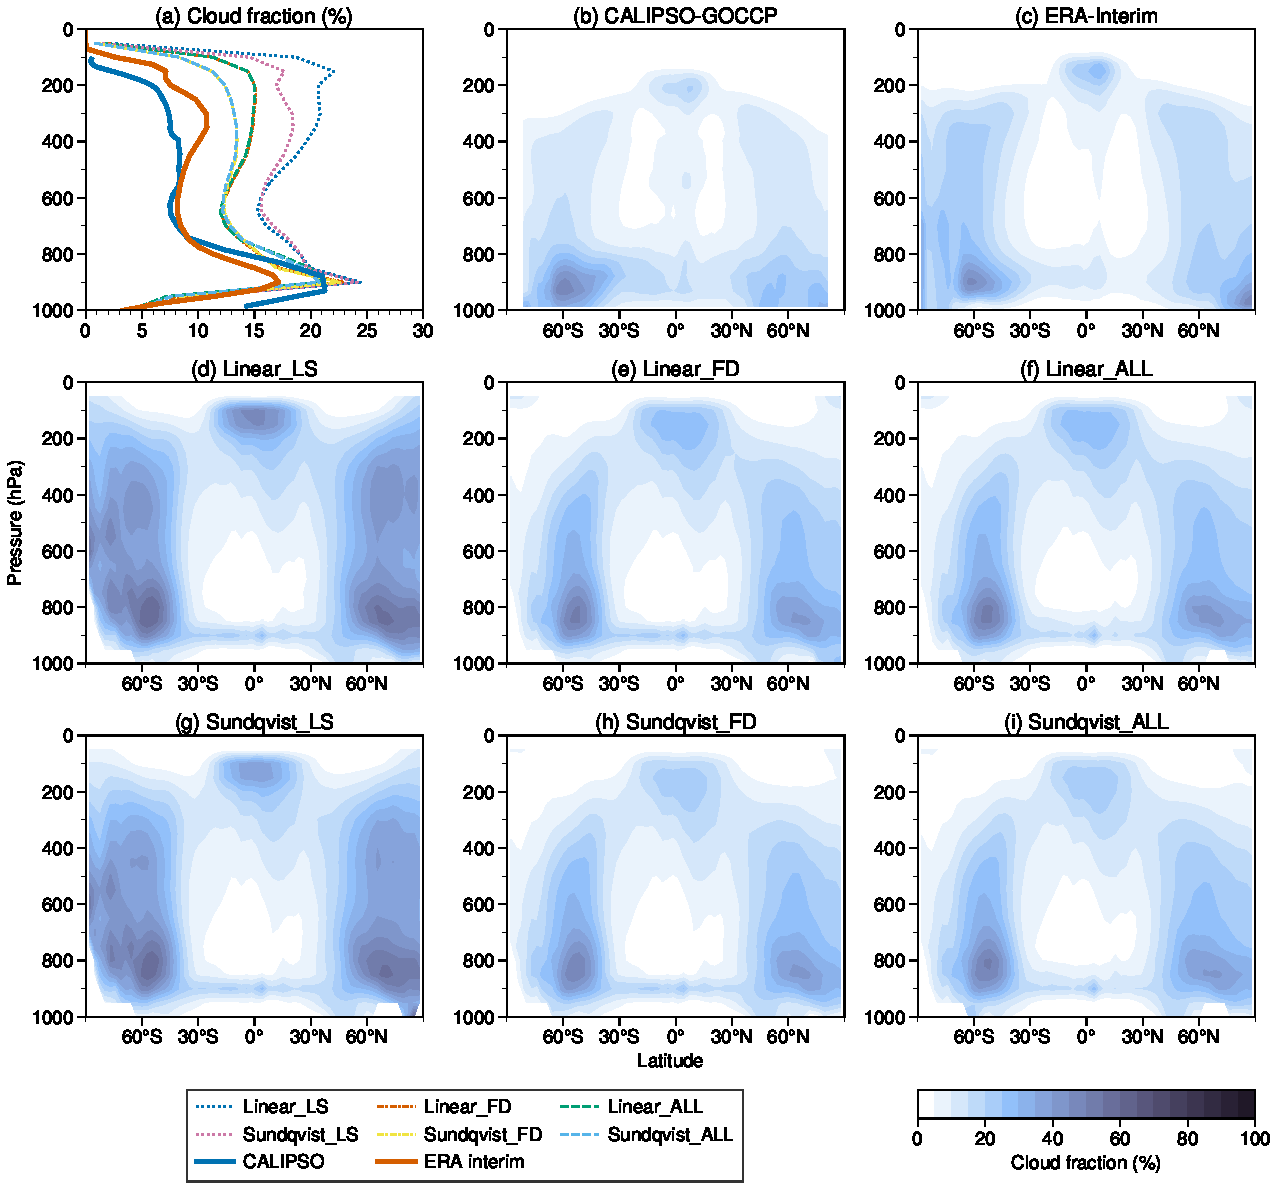
\includegraphics[width=1.\linewidth]{{figs/evaluation_of_cld_scheme/cloud_zonal_mean_vert_profiles}.pdf}
	\caption{(a) The annual and global mean of cloud fraction profiles from the CALIPSO-GOCCP (thick blue solid line), ERA-Interim reanalysis (thick orange solid line) and different Isca simulations, including linear\_LS (blue dotted), linear\_FD (orange dash-dotted), linear\_ALL (green dashed), Sundqvist\_LS (pink dotted), Sundqvist\_FD (yellow dash-dotted) and Sundqvist\_ALL (azure dashed). (b-i) Same as in (a), but for annual and zonal mean of cloud fraction profiles.}
	\label{fig:cld_fraction_profile}
\end{figure}

The global mean cloud fraction profiles from CALIPSO-GOCCP, ERA-Interim reanalysis and Isca simulations are displayed in \figref{fig:cld_fraction_profile}a. The cloud fractions from all the Isca simulations are higher than observations, especially in the middle and high levels. The FD simulations are closer to observations than the LS simulations, which is true for both the linear and Sundqvist schemes. Regarding the annual and zonal mean profiles, a striking feature is that the LS simulations from both linear and Sundqvist schemes overestimate the cloud fraction at high latitudes (\figsref{fig:cld_fraction_profile}d and \ref{fig:cld_fraction_profile}g) compared to the observation (\figref{fig:cld_fraction_profile}b) and reanalysis (\figref{fig:cld_fraction_profile}c). These biases are mitigated in the FD simulations (\figsref{fig:cld_fraction_profile}e and \ref{fig:cld_fraction_profile}h), as the cloud fractions are limited due to insufficient water vapor content at high latitudes. Despite more clouds being diagnosed at low levels over the eastern subtropical ocean regions, the zonal mean cloud fraction profiles in the ALL simulations (\figsref{fig:cld_fraction_profile}f and \ref{fig:cld_fraction_profile}i) are generally similar to those from the FD simulations. In summary, the cloud fraction profiles have been improved from the LS to ALL simulations due to the freeze-dry adjustment and the extra low clouds. However, the cloud fractions are still overestimated in high levels over the subtropics, which could possibly explain the CRE biases over these regions.


\section{Simulated cloud water path}


\section{Simulated cloud radiative effect}

\section{Comparison with CMIP5 models}

\section{Discussion and conclusions}

